\documentclass[11pt,a4paper]{article}

% ─── Packages ────────────────────────────────────────────────────────────────
\usepackage[utf8]{inputenc}
\usepackage[T1]{fontenc}
\usepackage{lmodern}
\usepackage[english]{babel}
\usepackage{geometry}
\geometry{margin=2.5cm, headheight=14.5pt}
\usepackage{graphicx}
\usepackage{xcolor}
\usepackage{hyperref}
\usepackage{listings}
\usepackage{booktabs}
\usepackage{longtable}
\usepackage{tabularx}
\usepackage{enumitem}
\usepackage{amsmath}
\usepackage{amssymb}
\usepackage{tikz}
\usetikzlibrary{shapes.geometric, arrows.meta, positioning, fit, calc, backgrounds}
\usepackage{fancyhdr}
\usepackage{titlesec}
\usepackage{tcolorbox}
\tcbuselibrary{skins,breakable}
\usepackage{float}
\usepackage{caption}
\usepackage{subcaption}
\usepackage{array}
\usepackage{multirow}
\usepackage{setspace}
\usepackage{parskip}

% ─── Star rating command ─────────────────────────────────────────────────────
\newcommand{\stars}[1]{%
  \ifnum#1>0\relax\ensuremath{\bigstar}\fi%
  \ifnum#1>1\relax\ensuremath{\bigstar}\fi%
  \ifnum#1>2\relax\ensuremath{\bigstar}\fi%
  \ifnum#1>3\relax\ensuremath{\bigstar}\fi%
  \ifnum#1>4\relax\ensuremath{\bigstar}\fi%
}

% ─── Section numbering depth ─────────────────────────────────────────────────
\setcounter{secnumdepth}{3}
\setcounter{tocdepth}{3}

% ─── Colours ─────────────────────────────────────────────────────────────────
\definecolor{phantomblue}{RGB}{30,90,180}
\definecolor{phantomgray}{RGB}{60,60,60}
\definecolor{codebg}{RGB}{245,245,250}
\definecolor{critred}{RGB}{200,30,30}
\definecolor{highorg}{RGB}{220,120,20}
\definecolor{medyel}{RGB}{180,160,0}
\definecolor{lowgrn}{RGB}{50,150,50}
\definecolor{layerbg}{RGB}{235,240,255}

% ─── Listings ────────────────────────────────────────────────────────────────
\lstset{
  basicstyle=\ttfamily\small,
  backgroundcolor=\color{codebg},
  frame=single,
  rulecolor=\color{gray!40},
  breaklines=true,
  numbers=left,
  numberstyle=\tiny\color{gray},
  keywordstyle=\color{phantomblue}\bfseries,
  commentstyle=\color{gray},
  stringstyle=\color{critred},
  showstringspaces=false,
  tabsize=4,
  captionpos=b,
}

% ─── Hyperref ────────────────────────────────────────────────────────────────
\hypersetup{
  colorlinks=true,
  linkcolor=phantomblue,
  urlcolor=phantomblue,
  citecolor=phantomblue,
  pdfauthor={Gadouri Rodwan},
  pdftitle={Phantom: Autonomous Adversary Simulation Platform},
  pdfsubject={System Documentation and Technical Guide},
}

% ─── Header / Footer ────────────────────────────────────────────────────────
\pagestyle{fancy}
\fancyhf{}
\rhead{\small\textcolor{gray}{Phantom v0.9.38 --- Documentation \& Guide}}
\lhead{\small\textcolor{gray}{\leftmark}}
\cfoot{\thepage}

% ─── tcolorbox environments ─────────────────────────────────────────────────
\newtcolorbox{infobox}[1][]{
  colback=blue!5, colframe=phantomblue, fonttitle=\bfseries,
  title=#1, breakable,
}
\newtcolorbox{warnbox}[1][]{
  colback=red!5, colframe=critred, fonttitle=\bfseries,
  title=#1, breakable,
}
\newtcolorbox{tipbox}[1][]{
  colback=green!5, colframe=lowgrn, fonttitle=\bfseries,
  title=#1, breakable,
}

% ─── TikZ styles (global) ───────────────────────────────────────────────────
\tikzset{
  block/.style={rectangle, draw=phantomblue, fill=blue!8, text width=3.2cm,
    minimum height=1cm, align=center, rounded corners=3pt, font=\small},
  bigblock/.style={rectangle, draw=phantomblue!60, fill=blue!3,
    minimum height=1cm, align=center, rounded corners=3pt, font=\small},
  pstep/.style={rectangle, draw=phantomblue, fill=blue!8, text width=4cm,
    minimum height=0.8cm, align=center, rounded corners=3pt, font=\small},
  decide/.style={diamond, draw=highorg, fill=orange!8, aspect=1.6,
    align=center, font=\small, inner sep=2pt},
  phase/.style={rectangle, draw=phantomblue, fill=blue!8, text width=3.5cm,
    minimum height=1.2cm, align=center, rounded corners=5pt, font=\small\bfseries},
  layer/.style={rectangle, draw=phantomblue!50, fill=layerbg,
    text width=14.5cm, minimum height=0.7cm, align=center, font=\footnotesize,
    rounded corners=2pt},
  arr/.style={-{Stealth[length=2.5mm]}, thick, phantomblue},
  arrdash/.style={-{Stealth[length=2.5mm]}, thick, phantomblue, dashed},
}


% ═══════════════════════════════════════════════════════════════════════════════
\begin{document}

% ─── Title Page ──────────────────────────────────────────────────────────────
\begin{titlepage}
\centering
\vspace*{2cm}
{\Huge\bfseries\textcolor{phantomblue}{Phantom}\par}
\vspace{0.5cm}
{\LARGE Autonomous Adversary Simulation Platform\par}
\vspace{0.3cm}
{\large System Documentation \& Technical Guide\par}
\vspace{1.5cm}
{\Large Version 0.9.38\par}
\vspace{0.5cm}
{\large March 2026\par}
\vspace{3cm}
\begin{tabular}{rl}
\textbf{Author:}      & Gadouri Rodwan \\[4pt]
\textbf{Supervisor:}   & Dr.\ Allama Oussama \\[4pt]
\textbf{Repository:}   & \url{https://github.com/Usta0x001/Phantom} \\[4pt]
\textbf{License:}      & Apache 2.0 \\
\end{tabular}
\vfill
{\small\textcolor{gray}{Open Source --- Apache 2.0 License}}
\end{titlepage}

% ─── Abstract ────────────────────────────────────────────────────────────────
\begin{abstract}
\noindent
Phantom is an AI-powered autonomous penetration testing platform that leverages
Large Language Models (LLMs) to discover, exploit, and verify real-world
vulnerabilities in web applications, APIs, and network services --- entirely
without human intervention. Unlike signature-based scanners that match known
patterns, Phantom employs a \textbf{ReAct} (Reason + Act) agent loop that reads HTTP
responses, reasons about attack surfaces, chains multi-step exploits, and
produces working proof-of-concept code.

This document serves as the \textbf{complete technical documentation and user guide}
for the Phantom system. It covers architecture, design philosophy, implementation
details, security controls, scanning workflows, LLM integration, the full tool
ecosystem, quality assurance, and deployment instructions.

\medskip\noindent
\textbf{Key result:} Against the OWASP Juice Shop benchmark (100+ known vulns),
Phantom v0.9.38 discovered 7 vulnerabilities (5~Critical, 2~High) in 26
iterations over 15 minutes at a cost of \$0.36.
\end{abstract}

\tableofcontents
\newpage

% ═══════════════════════════════════════════════════════════════════════════════
\section{Introduction}
\label{sec:intro}

\subsection{Motivation}
Traditional penetration testing is expensive, time-consuming, and suffers from
a critical talent shortage. According to (ISC)\textsuperscript{2}, the global
cybersecurity workforce gap exceeds 3.4~million professionals. Automated
scanners like Nessus, Burp Suite, and OWASP ZAP address only known
vulnerability signatures, missing business logic flaws, chained exploits, and
novel attack vectors that require human-like reasoning.

Phantom bridges this gap by combining the reasoning capabilities of frontier
LLMs with a rich toolkit of offensive security instruments, all operating within
a sandboxed Docker environment. The system autonomously:
\begin{enumerate}[noitemsep]
  \item Reconnoitres the target (port scanning, web crawling, technology fingerprinting)
  \item Discovers attack surfaces (endpoints, parameters, authentication flows)
  \item Exploits vulnerabilities with working PoC payloads
  \item Verifies findings through multiple confirmation strategies
  \item Generates structured reports with CVSS scoring, MITRE ATT\&CK mappings, and compliance mapping
\end{enumerate}

\subsection{Objectives}
\begin{itemize}[noitemsep]
  \item Design and implement an autonomous adversary simulation agent
  \item Achieve parity with or exceed manual penetration testing for common web vulnerabilities
  \item Ensure safe operation through defence-in-depth (sandboxing, scope validation, cost control)
  \item Provide actionable, standards-compliant vulnerability reports
  \item Support multiple LLM providers for flexibility and cost optimisation
\end{itemize}

\subsection{Scope}
Phantom targets:
\begin{itemize}[noitemsep]
  \item Web applications (black-box and grey-box)
  \item REST / GraphQL APIs
  \item Network services (via Nmap)
  \item Source code repositories (static analysis via Semgrep)
\end{itemize}

\subsection{At a Glance (v0.9.38)}
\begin{table}[H]
\centering
\caption{Phantom v0.9.38 metrics}
\label{tab:metrics}
\begin{tabular}{lr}
\toprule
\textbf{Metric} & \textbf{Value} \\
\midrule
Python source files           & 124 \\
Lines of Python code          & $\sim$31{,}900 \\
Registered security tools     & 55  \\
Scan profiles                 & 5   \\
Test cases (passing)          & 731 \\
Test cases (skipped)          & 97  \\
System prompt length          & 407 lines \\
Defence layers                & 11 \\
LLM providers supported       & 7+ \\
License                       & Apache 2.0 \\
Minimum Python version        & 3.12 \\
\bottomrule
\end{tabular}
\end{table}


% ═══════════════════════════════════════════════════════════════════════════════
\section{System Architecture}
\label{sec:arch}

\subsection{Design Philosophy}
Phantom is built on four core principles:

\begin{enumerate}
  \item \textbf{LLM-guided reasoning over signature matching} --- The agent reads
        responses, identifies attack surfaces, and chains exploits using natural
        language understanding rather than pattern databases.
  \item \textbf{Verify before report} --- Every finding must have a working PoC.
        Unverified findings are flagged but never falsely promoted.
  \item \textbf{Sandbox-first execution} --- All offensive tools run inside ephemeral
        Docker containers with no host network access, no privilege escalation,
        and restricted capabilities.
  \item \textbf{Never lose data} --- The findings ledger survives memory compression.
        HMAC-chained audit trails use \texttt{fsync} for crash safety.
\end{enumerate}

\subsection{High-Level Architecture}

Figure~\ref{fig:arch} shows how Phantom's components interact. The user (or CI
pipeline) provides a target through the CLI. The \textbf{PhantomAgent} orchestrates
everything: it queries the LLM for reasoning, dispatches tool calls through
the \textbf{Tool Executor}, and tracks all state. Offensive tools run inside an
ephemeral \textbf{Docker Sandbox} (Kali Linux) for isolation. Security controls
and the post-scan enrichment pipeline operate on the host side.

\begin{figure}[H]
\centering
\resizebox{\textwidth}{!}{
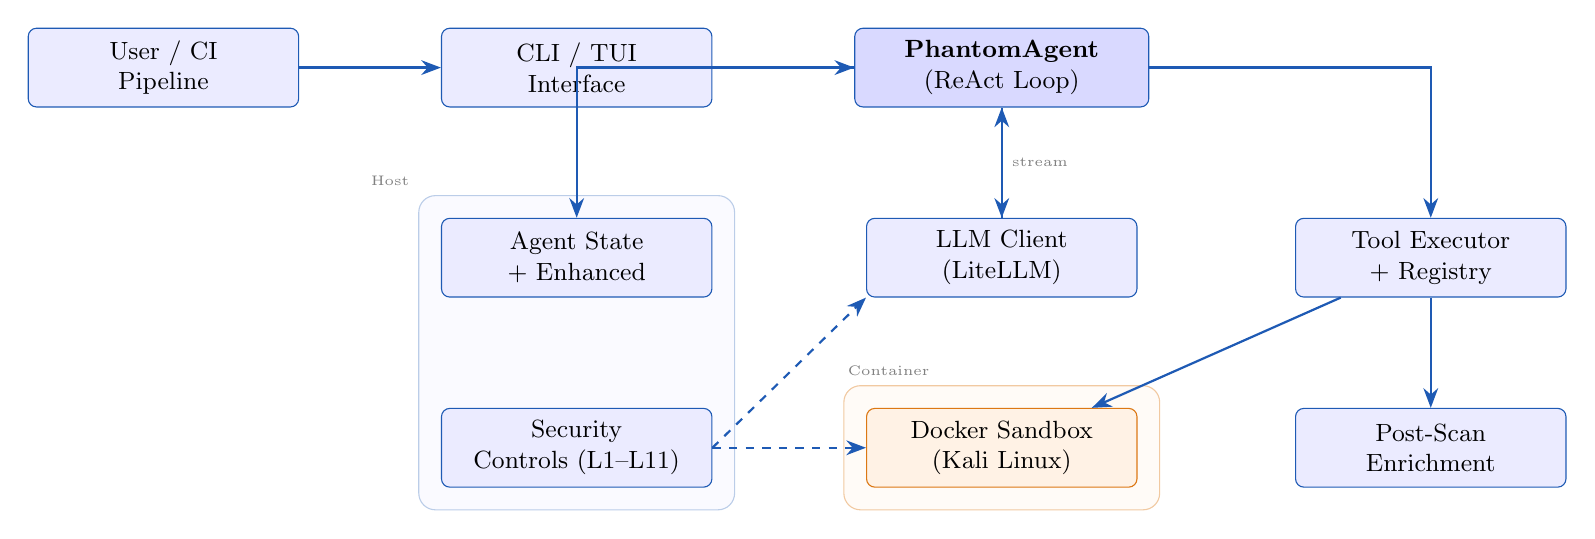
\begin{tikzpicture}[
  node distance=1.4cm and 1.8cm,
]

% ── Row 1: User → CLI → Agent ──
\node[block] (user) {User / CI\\Pipeline};
\node[block, right=of user] (cli) {CLI / TUI\\Interface};
\node[block, right=of cli, text width=3.5cm, fill=blue!15] (agent) {\textbf{PhantomAgent}\\(ReAct Loop)};

% ── Row 2: State | LLM | Executor ──
\node[block, below=of cli] (state) {Agent State\\+ Enhanced};
\node[block, below=of agent] (llm) {LLM Client\\(LiteLLM)};
\node[block, right=2cm of llm] (exec) {Tool Executor\\+ Registry};

% ── Row 3: Security | Sandbox | PostScan ──
\node[block, below=of state] (security) {Security\\Controls (L1--L11)};
\node[block, below=of llm, fill=orange!10, draw=highorg] (sandbox) {Docker Sandbox\\(Kali Linux)};
\node[block, below=of exec] (finish) {Post-Scan\\Enrichment};

% ── Arrows ──
\draw[arr] (user) -- (cli);
\draw[arr] (cli) -- (agent);
\draw[arr] (agent) -- (llm);
\draw[arr] (agent) -| (state);
\draw[arr] (agent) -| (exec);
\draw[arr] (exec) -- (sandbox);
\draw[arr] (exec) -- (finish);
\draw[arr] (llm) -- node[right, font=\tiny, text=gray]{stream} (agent);
\draw[arrdash] (security) -- (sandbox);
\draw[arrdash] (security.east) -- (llm.south west);

% ── Grouping box ──
\begin{scope}[on background layer]
  \node[fit=(state)(security), draw=phantomblue!30, fill=blue!2,
        rounded corners=6pt, inner sep=8pt, label={[font=\tiny\color{gray}]above left:Host}] {};
  \node[fit=(sandbox), draw=highorg!40, fill=orange!3,
        rounded corners=6pt, inner sep=8pt, label={[font=\tiny\color{gray}]above left:Container}] {};
\end{scope}

\end{tikzpicture}
}
\caption{Phantom high-level architecture. Solid arrows show data flow;
  dashed arrows show security enforcement boundaries.}
\label{fig:arch}
\end{figure}

\subsection{Package Structure}
\begin{table}[H]
\centering
\caption{Phantom package organisation}
\label{tab:packages}
\begin{tabularx}{\textwidth}{lX}
\toprule
\textbf{Package} & \textbf{Purpose} \\
\midrule
\texttt{phantom.agents}    & Agent core: ReAct loop, state machine, PhantomAgent persona \\
\texttt{phantom.core}      & Security \& domain logic: 17 modules including scope validation, verification, audit logging \\
\texttt{phantom.tools}     & Tool implementations: 15 subdirectories, 55 registered tools \\
\texttt{phantom.llm}       & LLM integration: client, provider registry, memory compressor, config \\
\texttt{phantom.runtime}   & Docker sandbox lifecycle and HTTP tool-server communication \\
\texttt{phantom.models}    & Pydantic domain models: Vulnerability, Host, ScanResult, ScanProfile \\
\texttt{phantom.skills}    & Markdown knowledge base: 9 vulnerability categories loaded into system prompt \\
\texttt{phantom.interface}  & CLI (Typer) and TUI (Rich) user interfaces \\
\texttt{phantom.telemetry}  & Observability: tracer, vulnerability report aggregation \\
\texttt{phantom.config}     & Configuration management with OS keyring support \\
\texttt{phantom.utils}      & Shared utilities \\
\bottomrule
\end{tabularx}
\end{table}


% ═══════════════════════════════════════════════════════════════════════════════
\section{Agent Architecture}
\label{sec:agent}

\subsection{The ReAct Loop}
Phantom's core engine implements a \textbf{Reason + Act} (ReAct) loop, a paradigm
where the agent alternates between thinking about observations and taking actions
via tool calls. The implementation resides in \texttt{base\_agent.py} (824~lines).

\begin{figure}[H]
\centering
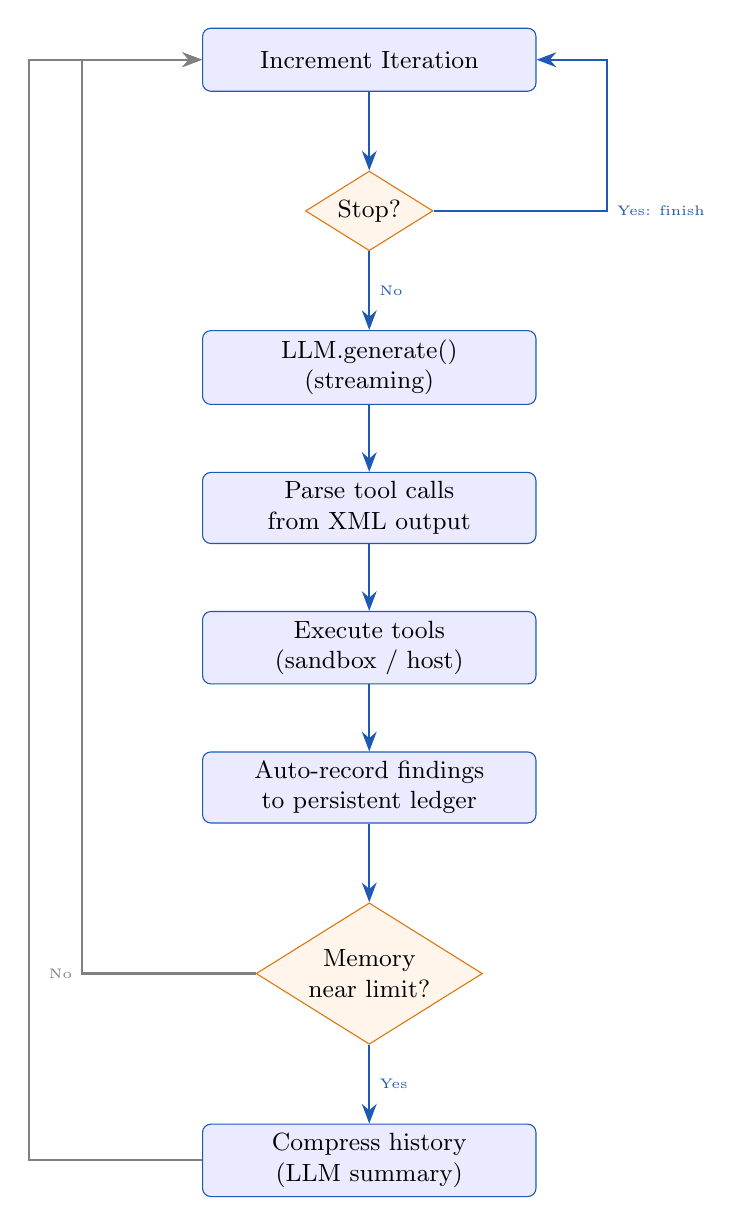
\begin{tikzpicture}[node distance=0.85cm]

\node[pstep] (start) {Increment Iteration};
\node[decide, below=1cm of start] (check) {Stop?};
\node[pstep, below=1cm of check] (llm) {LLM.generate()\\(streaming)};
\node[pstep, below=of llm] (parse) {Parse tool calls\\from XML output};
\node[pstep, below=of parse] (exec) {Execute tools\\(sandbox / host)};
\node[pstep, below=of exec] (record) {Auto-record findings\\to persistent ledger};
\node[decide, below=1cm of record] (compress) {Memory\\near limit?};
\node[pstep, below=1cm of compress] (comp) {Compress history\\(LLM summary)};

\draw[arr] (start) -- (check);
\draw[arr] (check) -- node[right, font=\tiny]{No} (llm);
\draw[arr] (llm) -- (parse);
\draw[arr] (parse) -- (exec);
\draw[arr] (exec) -- (record);
\draw[arr] (record) -- (compress);
\draw[arr] (compress) -- node[right, font=\tiny]{Yes} (comp);

% Loop-back arrows
\draw[arr] (check.east) -- ++(2.2,0)
  node[right, font=\tiny]{Yes: finish}
  |- (start.east);
\draw[arr, gray] (compress.west) -- ++(-2.2,0)
  node[left, font=\tiny, text=gray]{No}
  |- (start.west);
\draw[arr, gray] (comp.west) -- ++(-2.2,0) |- (start.west);

\end{tikzpicture}
\caption{The ReAct loop workflow. Each iteration queries the LLM, executes
  the requested tools, records findings, and optionally compresses
  conversation history when approaching the context window limit.}
\label{fig:react}
\end{figure}

\subsection{Stop Conditions}
The agent loop terminates when any of these conditions is met:
\begin{itemize}[noitemsep]
  \item \textbf{Iteration cap}: $\text{iteration} \geq \text{max\_iterations}$ (default: 300)
  \item \textbf{Completion}: Agent calls \texttt{finish\_scan} tool
  \item \textbf{User abort}: \texttt{stop\_requested} flag (Ctrl+C)
  \item \textbf{Cost limit}: Budget exceeded (\$25 default)
  \item \textbf{LLM failure}: After exhausting all retries
\end{itemize}

\subsection{Approaching-Max Warning}
At 85\% of \texttt{max\_iterations} (configurable threshold), the agent receives a
system warning to prioritise high-value findings. At $\text{max}-3$ iterations, a
final wrap-up message is injected (guarded: only fires when $\text{max} > 3$).

\subsection{Agent State}
\texttt{AgentState} (268~lines) is a Pydantic model tracking:
\begin{itemize}[noitemsep]
  \item Conversation history (max 500 messages)
  \item Findings ledger (immune to memory compression)
  \item Unverified findings queue
  \item Actions taken and observations (max 5{,}000 each)
  \item Iteration counter, phase, timing, cost accumulation
\end{itemize}

\texttt{EnhancedAgentState} (553~lines) extends this with:
\begin{itemize}[noitemsep]
  \item Vulnerability tracking (\texttt{dict[str, Vulnerability]})
  \item Host/service enumeration
  \item Endpoint tracking with deduplication (capped at 10{,}000)
  \item CVSS-based priority queues
  \item Checkpoint save/restore for scan resume
  \item Knowledge store integration for false-positive filtering
\end{itemize}

\subsection{System Prompt}
The system prompt is a 407-line Jinja2 template defining the agent's persona,
capabilities, communication rules, and vulnerability focus areas. It dynamically
loads security skill documents based on the target type.

\subsubsection{Vulnerability Focus Areas}
\begin{enumerate}[noitemsep]
  \item IDOR (Insecure Direct Object References)
  \item SQL Injection
  \item Server-Side Request Forgery (SSRF)
  \item Cross-Site Scripting (XSS)
  \item XML External Entity (XXE)
  \item Remote Code Execution (RCE)
  \item Cross-Site Request Forgery (CSRF)
  \item Race Conditions
  \item Business Logic Flaws
  \item Authentication \& JWT Weaknesses
\end{enumerate}


% ═══════════════════════════════════════════════════════════════════════════════
\section{LLM Integration}
\label{sec:llm}

\subsection{Client Architecture}
The LLM client (\texttt{llm.py}, 454~lines) is built on \textbf{LiteLLM}, providing
a unified interface to 100+ LLM providers. Key features:
\begin{itemize}[noitemsep]
  \item \textbf{Streaming}: Processes responses chunk-by-chunk, stops at
        \texttt{</function>} tag
  \item \textbf{Dynamic context window}: Reads model's actual context window from
        provider registry; sets compression threshold at 75\%
  \item \textbf{Retry with exponential backoff}: Up to 5 retries; wait =
        $\min(10,\; 2 \cdot 2^{n}) + \text{jitter}$
  \item \textbf{Cost tracking}: Per-request \texttt{RequestStats} with
        input/output/cached tokens and USD cost
  \item \textbf{Temperature}: \texttt{None} (uses model default) per v0.9.34
\end{itemize}

\subsection{Memory Compression}
When conversation history approaches the context window limit (75\% threshold),
the \texttt{MemoryCompressor} (448~lines) summarises older messages using a
specialised 10-rule prompt that preserves:
\begin{itemize}[noitemsep]
  \item Exact URLs, ports, endpoints, IP addresses
  \item Exact payloads, HTTP headers, cookies, credentials
  \item Full technology stack details
  \item All failed attempts (to avoid repetition)
  \item Attack surface maps and open ports
\end{itemize}

The findings ledger is \textbf{never compressed} --- it is injected into summaries
but maintained separately as a persistent record.

\subsection{Provider Registry}
Phantom ships with 18+ pre-configured model presets across 7~providers:

\begin{table}[H]
\centering
\caption{Pre-configured LLM providers}
\label{tab:providers}
\begin{tabularx}{\textwidth}{lX}
\toprule
\textbf{Provider} & \textbf{Models} \\
\midrule
Groq       & llama-3.3-70b-versatile, llama-3.1-8b-instant, llama3-70b-8192 \\
OpenAI     & gpt-4o (128K ctx), gpt-4o-mini \\
Anthropic  & claude-sonnet-4-20250514 (200K ctx), claude-3-5-haiku-latest \\
Google     & gemini-2.5-flash (1M ctx) \\
Ollama     & llama3:70b (local, free) \\
OpenRouter & deepseek-v3.2, deepseek-chat-v3-0324, gemini-2.5-flash, \\
           & llama-3.3-70b-instruct, gemma-3-27b-it:free, \\
           & hermes-3-llama-3.1-405b:free, qwen3-coder:free, \\
           & mistral-small-3.1-24b:free, grok-4.1-fast \\
\bottomrule
\end{tabularx}
\end{table}

\subsection{Fallback Chain}
The \texttt{FallbackChain} class provides automatic model failover. If the primary
model fails (rate limit, quota, outage), it advances to the next configured
provider, logging the transition and tracking failure counts.


% ═══════════════════════════════════════════════════════════════════════════════
\section{Tool Ecosystem}
\label{sec:tools}

\subsection{Registration \& Execution}
Tools are registered via the \texttt{@register\_tool} decorator with XML schema
files for parameter validation. The executor dispatches tools either to the
Docker sandbox (via HTTP) or locally, depending on the \texttt{sandbox\_execution}
flag.

\begin{figure}[H]
\centering
\resizebox{\textwidth}{!}{
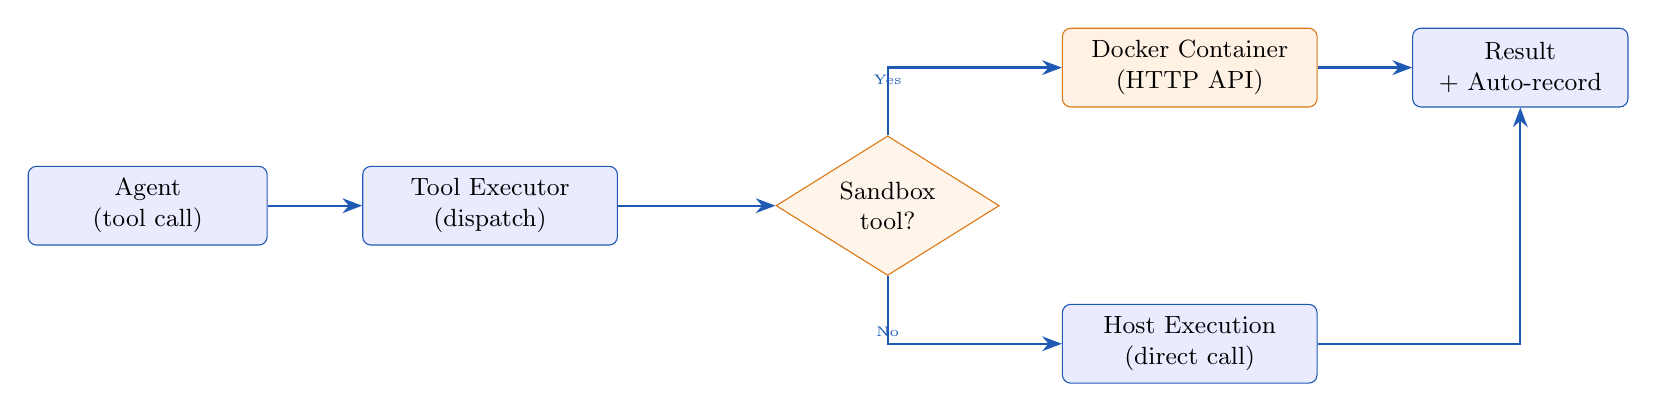
\begin{tikzpicture}[node distance=0.8cm and 1.2cm]
  \node[block, text width=2.8cm] (agent) {Agent\\(tool call)};
  \node[block, right=of agent, text width=3cm] (exec) {Tool Executor\\(dispatch)};
  \node[decide, right=2cm of exec, text width=1.5cm] (sandbox) {Sandbox\\tool?};
  \node[block, above right=0.8cm and 1.5cm of sandbox, text width=3cm, fill=orange!10, draw=highorg] (docker) {Docker Container\\(HTTP API)};
  \node[block, below right=0.8cm and 1.5cm of sandbox, text width=3cm] (local) {Host Execution\\(direct call)};
  \node[block, right=of docker, text width=2.5cm] (result) {Result\\+ Auto-record};

  \draw[arr] (agent) -- (exec);
  \draw[arr] (exec) -- (sandbox);
  \draw[arr] (sandbox) |- node[above, font=\tiny, pos=0.3]{Yes} (docker);
  \draw[arr] (sandbox) |- node[below, font=\tiny, pos=0.3]{No} (local);
  \draw[arr] (docker) -- (result);
  \draw[arr] (local) -| (result);
\end{tikzpicture}
}
\caption{Tool execution dispatch: sandbox tools run in the Docker container via
  HTTP; host-side tools (thinking, reporting, agent management) run locally.}
\label{fig:tool-dispatch}
\end{figure}

\subsection{Complete Tool Inventory}
{\small
\begin{longtable}{llp{5.5cm}}
\caption{All 55 registered tools} \label{tab:tools} \\
\toprule
\textbf{Category} & \textbf{Tool} & \textbf{Purpose} \\
\midrule
\endfirsthead
\multicolumn{3}{c}{\tablename\ \thetable\ --- continued} \\
\toprule
\textbf{Category} & \textbf{Tool} & \textbf{Purpose} \\
\midrule
\endhead
\bottomrule
\endfoot
Thinking    & \texttt{think}                    & Chain-of-thought reasoning \\
\midrule
\multirow{2}{*}{Nmap}
            & \texttt{nmap\_scan}               & Port scanning + service detection \\
            & \texttt{nmap\_vuln\_scan}          & Vulnerability script scanning \\
\midrule
\multirow{3}{*}{Nuclei}
            & \texttt{nuclei\_scan}             & Template-based vulnerability scanning \\
            & \texttt{nuclei\_scan\_cves}        & Known CVE detection \\
            & \texttt{nuclei\_scan\_misconfigs}  & Misconfiguration detection \\
\midrule
\multirow{3}{*}{SQLMap}
            & \texttt{sqlmap\_test}             & SQL injection detection \\
            & \texttt{sqlmap\_forms}            & Form-based SQLi testing \\
            & \texttt{sqlmap\_dump\_database}    & Database extraction \\
\midrule
\multirow{3}{*}{FFuf}
            & \texttt{ffuf\_directory\_scan}     & Directory brute-forcing \\
            & \texttt{ffuf\_parameter\_fuzz}     & Parameter discovery \\
            & \texttt{ffuf\_vhost\_fuzz}         & Virtual host enumeration \\
\midrule
\multirow{3}{*}{Httpx}
            & \texttt{httpx\_probe}             & HTTP probing + tech fingerprinting \\
            & \texttt{httpx\_screenshot}         & Screenshot capture \\
            & \texttt{httpx\_full\_analysis}     & Deep HTTP analysis \\
\midrule
Katana      & \texttt{katana\_crawl}            & Advanced web crawling \\
\midrule
\multirow{2}{*}{Subfinder}
            & \texttt{subfinder\_enumerate}     & Subdomain enumeration \\
            & \texttt{subfinder\_with\_sources}  & Subfinder with source tracking \\
\midrule
\multirow{3}{*}{Verification}
            & \texttt{verify\_vulnerability}     & Auto-verify via 8 strategies \\
            & \texttt{check\_known\_vulns}       & Query knowledge store \\
            & \texttt{enrich\_vulnerability}     & MITRE ATT\&CK + CWE mapping \\
\midrule
\multirow{5}{*}{Proxy}
            & \texttt{send\_request}            & Send HTTP request with auth injection \\
            & \texttt{repeat\_request}          & Replay captured request \\
            & \texttt{list\_requests}           & List captured traffic \\
            & \texttt{view\_request}            & View request/response details \\
            & \texttt{scope\_rules}             & Manage scope rules \\
\midrule
Terminal    & \texttt{terminal\_execute}         & Execute shell commands in sandbox \\
Python      & \texttt{python\_action}            & Run Python scripts in sandbox \\
Browser     & \texttt{browser\_action}           & Playwright browser automation \\
\midrule
\multirow{2}{*}{Reporting}
            & \texttt{create\_vulnerability\_report} & Detailed finding report (16+ params) \\
            & \texttt{report\_vulnerability}     & Quick finding report (5 params) \\
\midrule
Finish      & \texttt{finish\_scan}              & Finalise scan + enrichment pipeline \\
\midrule
\multirow{3}{*}{Agents}
            & \texttt{create\_agent}             & Spawn specialised sub-agent \\
            & \texttt{send\_message\_to\_agent}  & Inter-agent messaging \\
            & \texttt{agent\_finish}             & Sub-agent completion \\
\end{longtable}
}

\subsection{Auto-Recording Pipeline}
The executor automatically extracts and records findings from tool outputs:
\begin{itemize}[noitemsep]
  \item \textbf{Nuclei}: severity, template name, matched URL
  \item \textbf{Nmap}: open ports, services, OS fingerprinting
  \item \textbf{Katana}: discovered URLs, API endpoints, forms
  \item \textbf{SQLMap}: injection points, vulnerability confirmation
  \item \textbf{send\_request}: SQLi indicators, XSS reflections, sensitive data exposure
\end{itemize}

These findings survive memory compression and ensure critical discoveries are
never lost, even if the LLM forgets about them during long scans.


% ═══════════════════════════════════════════════════════════════════════════════
\section{Security Controls}
\label{sec:security}

\subsection{Defence-in-Depth Model}
Phantom implements 11 independent security layers. Each layer provides protection
even if other layers are bypassed.

\begin{figure}[H]
\centering
\resizebox{\textwidth}{!}{
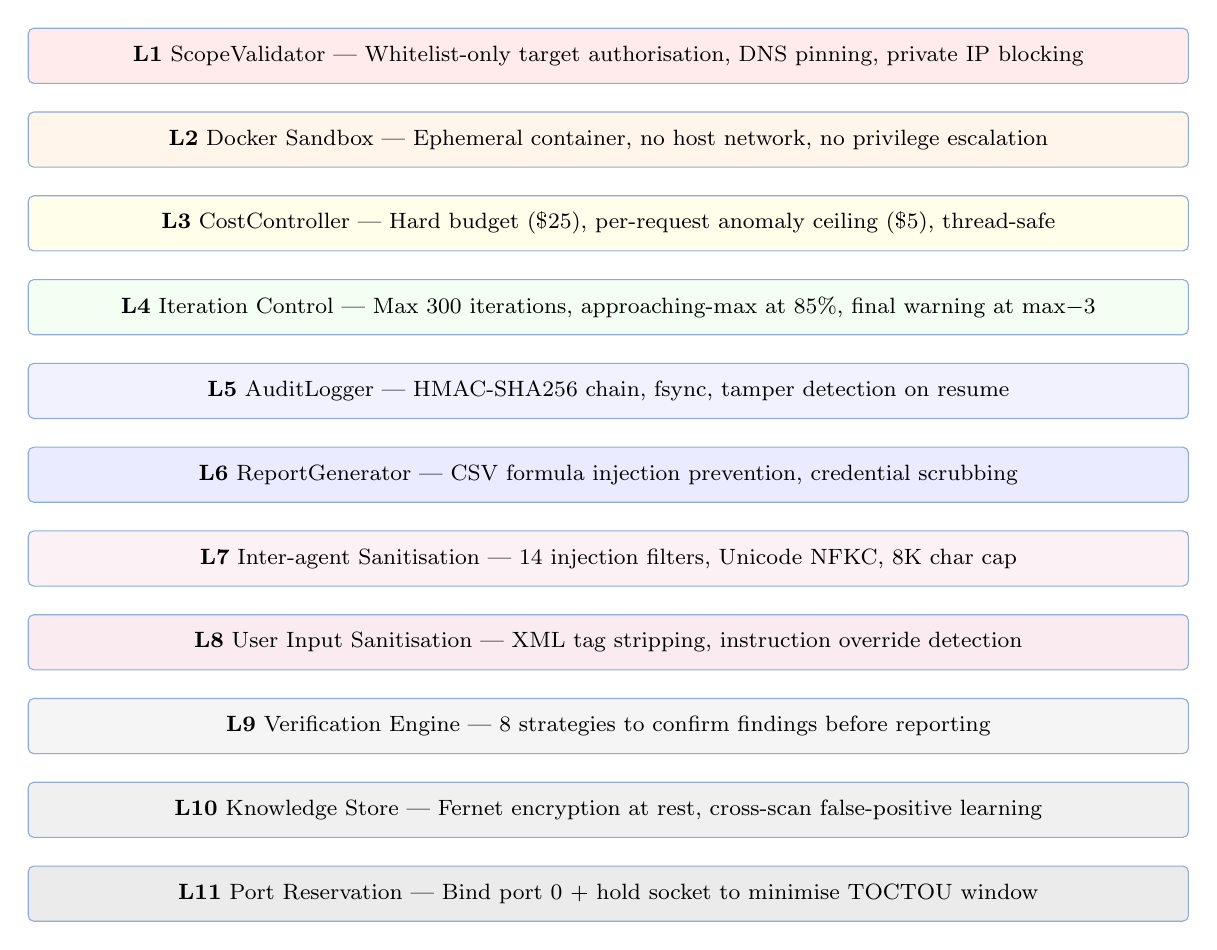
\begin{tikzpicture}[node distance=0.35cm]
  \node[layer, fill=red!8] (l1) {\textbf{L1} ScopeValidator --- Whitelist-only target authorisation, DNS pinning, private IP blocking};
  \node[layer, fill=orange!8, below=of l1] (l2) {\textbf{L2} Docker Sandbox --- Ephemeral container, no host network, no privilege escalation};
  \node[layer, fill=yellow!8, below=of l2] (l3) {\textbf{L3} CostController --- Hard budget (\$25), per-request anomaly ceiling (\$5), thread-safe};
  \node[layer, fill=green!5, below=of l3] (l4) {\textbf{L4} Iteration Control --- Max 300 iterations, approaching-max at 85\%, final warning at max$-$3};
  \node[layer, fill=blue!5, below=of l4] (l5) {\textbf{L5} AuditLogger --- HMAC-SHA256 chain, fsync, tamper detection on resume};
  \node[layer, fill=blue!8, below=of l5] (l6) {\textbf{L6} ReportGenerator --- CSV formula injection prevention, credential scrubbing};
  \node[layer, fill=purple!5, below=of l6] (l7) {\textbf{L7} Inter-agent Sanitisation --- 14 injection filters, Unicode NFKC, 8K char cap};
  \node[layer, fill=purple!8, below=of l7] (l8) {\textbf{L8} User Input Sanitisation --- XML tag stripping, instruction override detection};
  \node[layer, fill=gray!8, below=of l8] (l9) {\textbf{L9} Verification Engine --- 8 strategies to confirm findings before reporting};
  \node[layer, fill=gray!12, below=of l9] (l10) {\textbf{L10} Knowledge Store --- Fernet encryption at rest, cross-scan false-positive learning};
  \node[layer, fill=gray!16, below=of l10] (l11) {\textbf{L11} Port Reservation --- Bind port~0 + hold socket to minimise TOCTOU window};
\end{tikzpicture}
}
\caption{Phantom's 11-layer defence-in-depth model. Each layer provides
  independent protection.}
\label{fig:defence}
\end{figure}

\subsection{Scope Validator}
The \texttt{ScopeValidator} (370~lines) enforces target authorisation:
\begin{itemize}[noitemsep]
  \item 4 rule types: domain (with wildcards), IP, CIDR, regex
  \item Deny rules override allow rules
  \item DNS pin cache (max 10{,}000 entries) prevents rebinding attacks
  \item ReDoS protection: pattern cap 500 chars, target cap 2{,}048 chars
  \item Private IP blocking prevents SSRF to internal networks
\end{itemize}

\subsection{Audit Logger}
The \texttt{AuditLogger} (449~lines) creates a tamper-evident, crash-safe audit trail:
\begin{itemize}[noitemsep]
  \item JSONL format, one JSON object per line
  \item Each entry contains \texttt{\_prev\_hash} and \texttt{\_hmac} (HMAC-SHA256)
  \item Unique per-run key (\texttt{secrets.token\_hex(32)}), protected with \texttt{chmod 0o600}
  \item \texttt{os.fsync} after every write for crash safety
  \item Auto-rotation at 50~MB
  \item Chain verification on resume; logs tampering detection events
\end{itemize}

\subsection{Cost Controller}
\begin{table}[H]
\centering
\caption{Cost controller limits (all thread-safe with mutex lock)}
\label{tab:cost}
\begin{tabular}{lrl}
\toprule
\textbf{Limit} & \textbf{Default} & \textbf{Purpose} \\
\midrule
Total scan cost      & \$25.00    & Hard budget cap \\
Per-request cost     & \$5.00     & Anomaly detection \\
Input tokens         & 5{,}000{,}000  & Token ceiling \\
Output tokens        & 500{,}000  & Token ceiling \\
Compression calls    & 50         & Prevent compression spirals \\
Warning threshold    & 80\%       & Early alert \\
\bottomrule
\end{tabular}
\end{table}

\subsection{Verification Engine}
The \texttt{VerificationEngine} (602~lines) implements 8 confirmation strategies:
\begin{enumerate}[noitemsep]
  \item \textbf{Time-based}: SQLi SLEEP, RCE sleep with 4.5s threshold
  \item \textbf{Error-based}: SQL error pattern matching
  \item \textbf{Boolean-based}: Boolean injection comparison
  \item \textbf{DOM reflection}: XSS DOM reflection check
  \item \textbf{OOB HTTP}: Out-of-band callback via InteractshClient
  \item \textbf{OOB DNS}: Out-of-band DNS callback
  \item \textbf{Known file}: LFI verification via known file reads
  \item \textbf{Math eval}: SSTI math expression evaluation
\end{enumerate}

\begin{warnbox}[Important]
Failure to auto-verify does \textbf{not} mean the finding is a false positive.
Unverified HIGH/CRITICAL findings are flagged as \texttt{[UNVERIFIED]} but never discarded.
\end{warnbox}


% ═══════════════════════════════════════════════════════════════════════════════
\section{Scanning Workflow}
\label{sec:workflow}

\subsection{Scan Lifecycle}

\begin{figure}[H]
\centering
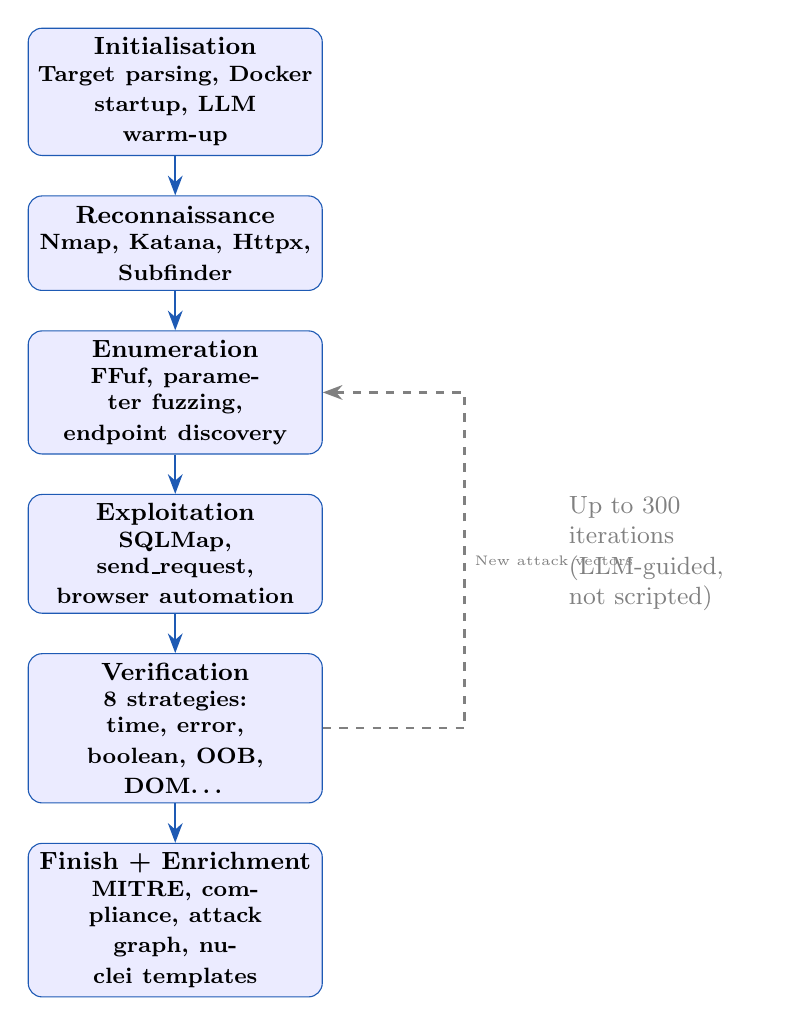
\begin{tikzpicture}[node distance=0.5cm]

\node[phase] (init) {Initialisation\\{\footnotesize Target parsing, Docker\\startup, LLM warm-up}};
\node[phase, below=of init] (recon) {Reconnaissance\\{\footnotesize Nmap, Katana, Httpx,\\Subfinder}};
\node[phase, below=of recon] (enum) {Enumeration\\{\footnotesize FFuf, parameter fuzzing,\\endpoint discovery}};
\node[phase, below=of enum] (exploit) {Exploitation\\{\footnotesize SQLMap, send\_request,\\browser automation}};
\node[phase, below=of exploit] (verify) {Verification\\{\footnotesize 8 strategies: time, error,\\boolean, OOB, DOM\ldots}};
\node[phase, below=of verify] (finish) {Finish + Enrichment\\{\footnotesize MITRE, compliance, attack\\graph, nuclei templates}};

\draw[arr] (init) -- (recon);
\draw[arr] (recon) -- (enum);
\draw[arr] (enum) -- (exploit);
\draw[arr] (exploit) -- (verify);
\draw[arr] (verify) -- (finish);

% Loop back
\draw[arrdash, gray] (verify.east) -- ++(1.8,0)
  |- node[right, font=\tiny\color{gray}, pos=0.25]{New attack vectors}
  (enum.east);

% Iteration counter
\node[right=3cm of exploit, font=\small\color{gray}, text width=2.5cm, align=left]
  {Up to 300\\iterations\\(LLM-guided,\\not scripted)};

\end{tikzpicture}
\caption{Scan lifecycle phases. The agent autonomously decides when to
  transition between phases based on its observations. The dashed loop-back
  arrow shows how new attack vectors discovered during verification can
  trigger additional enumeration.}
\label{fig:lifecycle}
\end{figure}

\subsection{Post-Scan Enrichment Pipeline}
When \texttt{finish\_scan} is called (minimum: 10 iterations + 8 tool calls),
a 6-stage enrichment pipeline executes:

\begin{enumerate}[noitemsep]
  \item \textbf{Verification} --- Re-exploits each finding via \texttt{VerificationEngine}
  \item \textbf{MITRE Enrichment} --- CWE, CAPEC, OWASP Top~10 mappings per finding
  \item \textbf{Compliance Mapping} --- OWASP/CWE/NIST/PCI DSS $\to$ \texttt{compliance\_report.md}
  \item \textbf{Attack Graph} --- NetworkX graph $\to$ \texttt{attack\_graph.json} + \texttt{attack\_paths.md}
  \item \textbf{Nuclei Templates} --- YAML templates for each finding $\to$ \texttt{nuclei\_templates/}
  \item \textbf{Knowledge Store} --- Persists vulns, hosts, history for cross-scan learning
\end{enumerate}

\subsection{Scan Profiles}
\begin{table}[H]
\centering
\caption{Available scan profiles}
\label{tab:profiles}
\begin{tabular}{lrrrll}
\toprule
\textbf{Profile} & \textbf{Iterations} & \textbf{Timeout} & \textbf{Memory} & \textbf{Browser} & \textbf{Special} \\
\midrule
Quick    & 300  & 120s & 120K & Yes & Skip subfinder \\
Standard & 120  & 120s & 80K  & Yes & Balanced \\
Deep     & 300  & 180s & 100K & Yes & All tools, sub-agents \\
Stealth  & 60   & 60s  & 60K  & No  & 2s delay, rate limit \\
API Only & 100  & 120s & 80K  & No  & No browser/subfinder \\
\bottomrule
\end{tabular}
\end{table}

\subsection{Scan Resume}
Phantom checkpoints state every 10 iterations to \texttt{checkpoint.json},
including iteration count, max\_iterations, phase, discovered hosts, endpoints,
vulnerabilities, and the findings ledger. Crashed scans can be resumed:
\begin{lstlisting}[language=bash]
phantom scan --resume <run-name>
\end{lstlisting}


% ═══════════════════════════════════════════════════════════════════════════════
\section{Configuration \& Deployment}
\label{sec:config}

\subsection{Environment Variables}
{\footnotesize
\begin{longtable}{p{4.5cm}p{1.5cm}p{6.5cm}}
\caption{Configuration environment variables} \label{tab:config} \\
\toprule
\textbf{Variable} & \textbf{Default} & \textbf{Description} \\
\midrule
\endfirsthead
\endhead
\bottomrule
\endfoot
\texttt{PHANTOM\_LLM}                    & (required)  & LLM model identifier (e.g.\ \texttt{openrouter/deepseek/deepseek-v3.2}) \\
\texttt{LLM\_API\_KEY}                   & ---         & API key for LLM provider \\
\texttt{PHANTOM\_LLM\_FALLBACK}          & ---         & Comma-separated fallback models \\
\texttt{PHANTOM\_MAX\_COST\_USD}          & 25.0        & Max LLM spend per scan \\
\texttt{PHANTOM\_LLM\_MAX\_RETRIES}       & 5           & Max retries per LLM request \\
\texttt{LLM\_TIMEOUT}                     & 300s        & LLM request timeout \\
\texttt{PHANTOM\_REASONING\_EFFORT}       & high        & LLM reasoning effort level \\
\texttt{PHANTOM\_SANDBOX\_IMAGE}          & ghcr.io/..  & Docker sandbox image \\
\texttt{PHANTOM\_SANDBOX\_EXECUTION\_TIMEOUT} & 600s   & Per-tool execution timeout \\
\texttt{PHANTOM\_DISABLE\_BROWSER}        & false       & Disable Playwright tools \\
\texttt{PHANTOM\_KNOWLEDGE\_KEY}          & ---         & Fernet key for knowledge store \\
\texttt{PHANTOM\_LOG\_LEVEL}              & INFO        & Logging verbosity \\
\end{longtable}
}

\subsection{Quick Start}
\begin{lstlisting}[language=bash,caption={Minimal setup to run Phantom}]
# 1. Install Phantom
pip install phantom-agent

# 2. Configure LLM (cheapest recommended option)
export PHANTOM_LLM="openrouter/deepseek/deepseek-v3.2"
export LLM_API_KEY="sk-or-v1-your-key-here"

# 3. Pull sandbox image
docker pull ghcr.io/usta0x001/phantom-sandbox:latest

# 4. Run a scan
phantom scan -t http://target.example.com -m quick
\end{lstlisting}

\subsection{Credential Storage}
Sensitive API keys use the \textbf{OS keyring} when available. A sentinel value
\texttt{\_\_KEYRING\_\_} is stored in the JSON config file, and the actual secret
is retrieved from the system credential store at runtime.

\subsection{Docker Sandbox}
The sandbox runs a \textbf{Kali Linux} container with pre-installed tools:
Nmap, Nuclei, SQLMap, FFuf, Httpx, Katana, Subfinder, Semgrep, Nikto,
Gobuster, Arjun, jwt\_tool, wafw00f, InteractSH, Playwright/Chromium,
Python~3, Node.js, and Go.

Communication occurs via an authenticated HTTP API on port 48081, secured
with a per-run \texttt{secrets.token\_urlsafe()} bearer token.

\subsection{Operating Modes}
\begin{table}[H]
\centering
\caption{Interactive vs.\ non-interactive modes}
\label{tab:modes}
\begin{tabularx}{\textwidth}{lXX}
\toprule
\textbf{Aspect} & \textbf{Interactive (TUI)} & \textbf{Non-Interactive (CLI)} \\
\midrule
Interface    & Rich Live dashboard with panels & Headless, log-only output \\
Invocation   & \texttt{phantom scan -t <url>} & \texttt{phantom scan -t <url> -n} \\
Completion   & User can send messages, Ctrl+C & Auto-exits when scan completes \\
Use Case     & Manual pen-testing, exploration & CI/CD pipelines, automation \\
TTY Required & Yes & No \\
\bottomrule
\end{tabularx}
\end{table}


% ═══════════════════════════════════════════════════════════════════════════════
\section{Quality Assurance}
\label{sec:qa}

\subsection{Test Suite}
As of v0.9.38:
\begin{itemize}[noitemsep]
  \item \textbf{731 tests passing}, 97 skipped (legacy-feature tests)
  \item Execution time: $\sim$74 seconds on commodity hardware
  \item Coverage areas: state management, security controls, tool execution,
        checkpoint/resume, memory compression, cost control, scope validation,
        report generation, inter-agent sanitisation
\end{itemize}

\subsection{Audit History}
\begin{table}[H]
\centering
\caption{Audit version history}
\label{tab:audit}
\begin{tabular}{lp{8cm}r}
\toprule
\textbf{Version} & \textbf{Key Changes} & \textbf{Tests} \\
\midrule
v0.9.32 & Sandbox startup fix (CRLF, sudoers, port reservation) & $\sim$700 \\
v0.9.33 & Auto-report pipeline, simplified reporting, phase fallback & $\sim$720 \\
v0.9.34 & Temperature=None, max\_iterations=300, VulnClassTracker disabled & $\sim$730 \\
v0.9.35 & 17 harmful diffs with legacy bloat removed & $\sim$735 \\
v0.9.36 & \textbf{CRITICAL}: Memory compression bug fix + deep cleanup ($-$4{,}050 lines) & 737 \\
v0.9.37 & Final audit: 9 fixes, dead code, docs, endpoint caps & 731 \\
v0.9.38 & Zero-base audit: 4~P0, 2~P1, 5~P2 fixes (race condition, auth leak, cost lock) & 731 \\
\bottomrule
\end{tabular}
\end{table}

\subsection{Benchmark Results}
\begin{table}[H]
\centering
\caption{OWASP Juice Shop benchmark comparison}
\label{tab:benchmark}
\begin{tabular}{lrrr}
\toprule
\textbf{Metric} & \textbf{v0.9.32} & \textbf{v0.9.38} & \textbf{$\Delta$} \\
\midrule
Vulnerabilities found   & 2       & 7 (5C + 2H) & +250\% \\
Iterations used         & 40      & 26           & $-$35\% \\
Scan time               & $\sim$5h & 15 min      & $-$95\% \\
Cost                    & $\sim$\$2 & \$0.36      & $-$82\% \\
\bottomrule
\end{tabular}
\end{table}


% ═══════════════════════════════════════════════════════════════════════════════
\section{LLM Selection Guide}
\label{sec:llmstudy}

\subsection{Requirements}
Phantom requires models that can:
\begin{enumerate}[noitemsep]
  \item Generate structured XML tool calls reliably
  \item Maintain long context (scans produce 50K--150K tokens of history)
  \item Reason about multi-step exploit chains
  \item Understand HTTP, SQL, JavaScript, and networking concepts
  \item Operate at reasonable cost (\$0.10--\$5.00 per scan)
\end{enumerate}

\subsection{Model Comparison}
{\small
\begin{longtable}{rlrrp{2.5cm}c}
\caption{LLM model comparison for Phantom (35 models across 6 tiers)} \label{tab:llmstudy} \\
\toprule
\textbf{\#} & \textbf{Model} & \textbf{Context} & \textbf{Cost/M in} & \textbf{Provider} & \textbf{Rating} \\
\midrule
\endfirsthead
\multicolumn{6}{c}{\tablename\ \thetable\ --- continued} \\
\toprule
\textbf{\#} & \textbf{Model} & \textbf{Context} & \textbf{Cost/M in} & \textbf{Provider} & \textbf{Rating} \\
\midrule
\endhead
\bottomrule
\endfoot

\multicolumn{6}{l}{\textbf{Tier~1: Recommended (Best Performance)}} \\
\midrule
1  & Claude Sonnet 4           & 200K   & \$3.00  & Anthropic        & \stars{5} \\
2  & GPT-4o                     & 128K   & \$2.50  & OpenAI           & \stars{5} \\
3  & DeepSeek V3.2              & 163K   & \$0.30  & OpenRouter       & \stars{5} \\
4  & Gemini 2.5 Flash           & 1M     & \$0.15  & Google/OpenRouter & \stars{5} \\
5  & Qwen3.5-122B               & 262K   & \$0.30  & OpenRouter       & \stars{4} \\
6  & DeepSeek Chat V3-0324      & 163K   & \$0.30  & OpenRouter       & \stars{4} \\
\midrule
\multicolumn{6}{l}{\textbf{Tier~2: Strong Alternatives}} \\
\midrule
7  & Grok 4.1 Fast              & 131K   & \$3.00  & xAI/OpenRouter   & \stars{4} \\
8  & Claude 3.5 Haiku           & 200K   & \$0.80  & Anthropic        & \stars{4} \\
9  & GPT-4o Mini                & 128K   & \$0.15  & OpenAI           & \stars{4} \\
10 & Qwen3.5-27B                & 262K   & \$0.27  & OpenRouter       & \stars{4} \\
11 & Qwen3.5-Flash              & 1M     & \$0.10  & OpenRouter       & \stars{4} \\
12 & Llama 3.3 70B              & 128K   & Free    & Groq             & \stars{4} \\
13 & Hermes 3 405B              & 131K   & Free    & OpenRouter       & \stars{3} \\
14 & Gemini 3.1 Flash Lite      & 1.05M  & \$0.25  & Google           & \stars{4} \\
\midrule
\multicolumn{6}{l}{\textbf{Tier~3: Budget / Free}} \\
\midrule
15 & Qwen3-Coder (free)         & 40K    & Free    & OpenRouter       & \stars{3} \\
16 & Gemma 3 27B (free)         & 96K    & Free    & OpenRouter       & \stars{3} \\
17 & Mistral Small 3.1 24B      & 128K   & Free    & OpenRouter       & \stars{3} \\
18 & Llama 3.1 8B               & 128K   & Free    & Groq             & \stars{2} \\
19 & Llama 3 70B 8192           & 8K     & Free    & Groq             & \stars{2} \\
20 & DeepSeek V3.1 Terminus     & 163K   & \$0.30  & OpenRouter       & \stars{3} \\
21 & LFM2-24B                   & 33K    & \$0.03  & Liquid/OpenRouter& \stars{2} \\
22 & ByteDance Seed 2.0 Mini    & 262K   & \$0.10  & OpenRouter       & \stars{3} \\
\midrule
\multicolumn{6}{l}{\textbf{Tier~4: Self-Hosted / Local}} \\
\midrule
23 & Llama 3:70b (Ollama)       & 8K     & Free    & Local            & \stars{3} \\
24 & Qwen2.5-72B (Ollama)       & 128K   & Free    & Local            & \stars{3} \\
25 & Mistral Large 2 (Ollama)   & 128K   & Free    & Local            & \stars{3} \\
26 & DeepSeek-R1-Distill        & 128K   & Free    & Local            & \stars{3} \\
27 & CodeLlama 70B              & 16K    & Free    & Local            & \stars{2} \\
\midrule
\multicolumn{6}{l}{\textbf{Tier~5: Premium / Enterprise}} \\
\midrule
28 & Claude Opus 4              & 200K   & \$15.00 & Anthropic        & \stars{5} \\
29 & GPT-4.5                    & 128K   & \$75.00 & OpenAI           & \stars{4} \\
30 & Gemini 2.5 Pro             & 1M     & \$1.25  & Google           & \stars{5} \\
31 & GPT-o3                     & 200K   & \$10.00 & OpenAI           & \stars{4} \\
32 & Grok 4.1                   & 131K   & \$6.00  & xAI              & \stars{4} \\
\midrule
\multicolumn{6}{l}{\textbf{Tier~6: Specialised / Niche}} \\
\midrule
33 & Mistral Codestral          & 256K   & \$0.30  & Mistral          & \stars{3} \\
34 & Cohere Command R+          & 128K   & \$2.50  & Cohere           & \stars{3} \\
35 & Fireworks Llama 3.3 70B    & 128K   & \$0.90  & Fireworks AI     & \stars{3} \\
\end{longtable}
}

\subsection{Recommendations}

\begin{tipbox}[Best Overall]
\textbf{DeepSeek V3.2} via OpenRouter --- \$0.30/M input, 163K context, excellent
tool-use. Proven: 7 vulns found at \$0.36/scan.
\end{tipbox}

\begin{tipbox}[Best Budget]
\textbf{Llama 3.3 70B} via Groq --- Free tier, 128K context. Fast inference via
Groq hardware. Ideal for development and testing.
\end{tipbox}

\begin{tipbox}[Best Premium]
\textbf{Claude Sonnet 4} --- 200K context, superior reasoning for complex exploit
chains. \$3/M justified for high-value targets.
\end{tipbox}

\begin{tipbox}[Best Context Window]
\textbf{Gemini 2.5 Flash} --- 1M context at \$0.15/M. Ideal for deep scans; the
1M window eliminates most compression needs.
\end{tipbox}

\begin{tipbox}[Best Self-Hosted]
\textbf{Qwen2.5-72B} via Ollama --- 128K context, free, runs on a single A100
GPU. Suitable for air-gapped environments.
\end{tipbox}


% ═══════════════════════════════════════════════════════════════════════════════
\section{Recommendations \& Future Work}
\label{sec:recommendations}

\subsection{System Quality Scores}
\begin{table}[H]
\centering
\caption{System quality assessment (v0.9.38)}
\label{tab:scores}
\begin{tabular}{lr}
\toprule
\textbf{Category} & \textbf{Score} \\
\midrule
Core Scan Engine        & 95/100 \\
LLM Integration         & 93/100 \\
Memory Management       & 95/100 \\
Security Hardening      & 92/100 \\
Post-Scan Enrichment    & 98/100 \\
Code Quality            & 90/100 \\
Documentation           & 88/100 \\
Test Coverage           & 87/100 \\
\midrule
\textbf{Overall}        & \textbf{92/100} \\
\bottomrule
\end{tabular}
\end{table}

\subsection{Predictions}
\begin{itemize}[noitemsep]
  \item A full 300-iteration scan on Juice Shop should find \textbf{15--25 vulnerabilities}
  \item Estimated cost per full scan: \textbf{\$1.50--\$3.00} with DeepSeek V3.2
  \item With Claude Sonnet 4: expect \textbf{20--30 vulnerabilities} at \$8--\$15/scan
  \item With Gemini 2.5 Flash: expect similar to DeepSeek at \textbf{60--80\% lower cost}
  \item v1.0 readiness: 2--3 more development cycles
\end{itemize}

\subsection{Short-Term Roadmap (v0.9.39--v0.9.41)}
\begin{enumerate}[noitemsep]
  \item \textbf{CI/CD Pipeline} --- GitHub Actions for automated testing on push
  \item \textbf{Benchmark Suite} --- Automated scans against DVWA, WebGoat, Juice Shop with regression tracking
  \item \textbf{SARIF Output} --- GitHub Code Scanning integration
  \item \textbf{Multi-Model Routing} --- Cheap model for recon, expensive for exploitation
\end{enumerate}

\subsection{Medium-Term (v0.10.x)}
\begin{enumerate}[noitemsep]
  \item \textbf{Parallel Tool Execution} --- Run independent tools concurrently
  \item \textbf{Agent Collaboration} --- Specialised sub-agents (recon, exploit, report)
  \item \textbf{Web Dashboard} --- Real-time scan monitoring via FastAPI + React
  \item \textbf{Plugin Marketplace} --- Community-contributed tools and skills
\end{enumerate}

\subsection{Long-Term (v1.0)}
\begin{enumerate}[noitemsep]
  \item \textbf{Autonomous Red Team Operations} --- Multi-target campaign management
  \item \textbf{Defensive Integration} --- WAF bypass testing, IDS evasion assessment
  \item \textbf{Compliance Automation} --- Full PCI DSS / SOC~2 vulnerability mapping
  \item \textbf{Enterprise Features} --- RBAC, multi-tenant, LDAP/SSO integration
\end{enumerate}

\subsection{Operator Guidelines}
\begin{enumerate}[noitemsep]
  \item Always run Phantom in a controlled environment with explicit authorisation
  \item Start with \texttt{quick} profile to validate setup before running \texttt{deep}
  \item Set \texttt{PHANTOM\_MAX\_COST\_USD} to prevent unexpected charges
  \item Review the audit log (\texttt{audit\_trail.jsonl}) after every scan
  \item Use \texttt{-{}-non-interactive} for CI/CD pipelines with \texttt{-{}-timeout}
  \item Keep the Docker image updated:\\
        {\small\texttt{docker pull ghcr.io/usta0x001/phantom-sandbox:latest}}
\end{enumerate}


% ═══════════════════════════════════════════════════════════════════════════════
\section{Conclusion}
\label{sec:conclusion}

Phantom v0.9.38 represents a mature, well-audited autonomous security scanning
platform that bridges the gap between signature-based vulnerability scanners and
human penetration testers. Through 8 rounds of deep audit (v0.9.32--v0.9.38),
the system has evolved from a prototype discovering 2 vulnerabilities into a
production-capable tool that finds 7+ vulnerabilities in minutes at sub-dollar
cost.

The architecture's strength lies in its clean separation between the reasoning
engine (LLM), the action layer (55 tools), and the safety controls (11 defence
layers). By aligning the core engine with the proven lean engine architecture while
retaining genuine Phantom innovations (verification engine, knowledge store,
attack graph, compliance mapping), the system achieves both raw scanning power
and enterprise-grade reporting.

\medskip
\noindent\textbf{Key contributions:}
\begin{itemize}[noitemsep]
  \item Demonstration that LLM-guided reasoning can match or exceed
        signature-based scanning for common web vulnerabilities
  \item A defence-in-depth framework ensuring safe autonomous operation
  \item A post-scan enrichment pipeline producing compliance-ready reports
  \item An extensible tool and skill system supporting future growth
  \item Support for 35+ LLM models across 7 providers with automatic fallback
\end{itemize}

\vspace{1cm}
\begin{center}
\textit{``The best security tool is the one that thinks like an attacker.''}
\end{center}


% ─── Glossary (Appendix) ────────────────────────────────────────────────────
\newpage
\appendix
\section{Glossary}
\begin{description}[noitemsep]
  \item[ReAct] Reason + Act --- agent paradigm alternating thinking and tool use
  \item[CVSS] Common Vulnerability Scoring System
  \item[IDOR] Insecure Direct Object Reference
  \item[SSRF] Server-Side Request Forgery
  \item[XSS] Cross-Site Scripting
  \item[SQLi] SQL Injection
  \item[RCE] Remote Code Execution
  \item[OOB] Out-of-Band (callback-based verification)
  \item[MITRE ATT\&CK] Adversary tactics and techniques knowledge base
  \item[OWASP] Open Web Application Security Project
  \item[LiteLLM] Python library for unified LLM API access
  \item[Jinja2] Python templating engine
  \item[PoC] Proof of Concept
  \item[SSTI] Server-Side Template Injection
  \item[JWT] JSON Web Token
  \item[HMAC] Hash-based Message Authentication Code
\end{description}

\section{Full Configuration Reference}
See Section~\ref{sec:config} for all environment variables. Additional options
are available in the \texttt{phantom config set} CLI command and the
\texttt{\textasciitilde/.phantom/cli-config.json} file.

\end{document}
